\documentclass[a4paper,12pt]{article}
\usepackage{geometry}
 \geometry{
 a4paper,
 total={170mm,257mm},
 left=20mm,
 top=20mm,
 }
\usepackage{adjustbox}
\usepackage[polish]{babel}
\usepackage{polski}
\usepackage{multirow}
\usepackage{makecell}
\usepackage{boldline}
\usepackage[T1]{fontenc} 
\usepackage{listings}
\usepackage{color}
\usepackage{biblatex}
\usepackage{csquotes}
\usepackage{indentfirst}
\addbibresource{doxygen.bib}

\lstset{literate={ą}{{\k{a}}}1 {ł}{{\l{}}}1 {ń}{{\'n}}1 {ę}{{\k{e}}}1 {ś}{{\'s}}1 {ż}{{\.z}}1 {ó}{{\'o}}1 {ź}{{\'z}}1 {Ą}{{\k{A}}}1 {Ł}{{\L{}}}1 {Ń}{{\'N}}1 {Ę}{{\k{E}}}1 {Ś}{{\'S}}1 {Ż}{{\.Z}}1 {Ó}{{\'O}}1 {Ź}{{\'Z}}1 {Ć}{{\'C}}1 {ć}{{\'c}}1 }

\title{Sprawozdanie z Zadania: Dokumentacja z doxygen}
\author{Jakub Kraus}
\date{24.01.2024}
\renewcommand\theadalign{tl}
\begin{document}
\renewcommand{\arraystretch}{2}
\begin{table}[ht]
    \centering
    \begin{adjustbox}{width=1\textwidth,center=\textwidth}
        \begin{tabular}{V{4}lV{4}c|c|c|c|c|c V{4}}
            \hlineB{4}
            \multicolumn{2}{V{4}lV{4}}{}                                         & \multicolumn{5}{lV{4}}{\textbf{Wydział Nauk Ścisłych i Technicznych}}                                                                                                                                   \\
            \cline{3-7}
            \multicolumn{2}{V{4}cV{4}}{\textbf{Uniwersytet Śląski w Katowicach}} & \multicolumn{5}{lV{4}}{\textbf{Instytut Fizyki}}                                                                                                                                                        \\
            \cline{3-7}
            \multicolumn{2}{V{4}lV{4}}{}                                         & Rok                                                                   & \textbf{III}                                          & Semestr                            & \multicolumn{2}{cV{4}}{\textbf{V}} \\
            \hlineB{4}
            Kierunek                                                             & \multicolumn{6}{cV{4}}{Informatyka stosowana}                                                                                                                                                           \\
            \hline
            Przedmiot                                                            & \multicolumn{6}{cV{4}}{\textbf{SiNWO - laboratorium}}                                                                                                                                                   \\
            \hlineB{4}
            Prowadzący                                                           & \multicolumn{6}{cV{4}}{dr Wojciech Gurdziel}                                                                                                                                                            \\
            \hline
            Tytuł ćwiczenia                                                      & \multicolumn{4}{c|}{\textbf{Automatyzacja generacji dokumentacji}}    &
            \multirow{2}{*}{Nr ćwiczenia}                                        & \multirow{2}{*}{\textbf{IV}}                                                                                                                                                                            \\
            \cline{1-5}
            \thead{Sprawozdanie wykonał:                                                                                                                                                                                                                                                   \\ (Imię i Nazwisko)} &
            \multicolumn{4}{c|}{\textbf{Jakub Kraus}}                            &                                                                       &                                                                                                                                 \\
            \hlineB{3}
            Data wykonania ćwiczenia                                             & \textbf{24.01.2024}                                                   & \multicolumn{2}{V{4}lV{4}}{Data oddania sprawozdania} & \multicolumn{3}{cV{4}}{01.02.2024}                                      \\
            \hlineB{4}
        \end{tabular}
    \end{adjustbox}
\end{table}
\newpage
\tableofcontents
\listoffigures
\lstlistoflistings
\newpage
\section{Cel ćwiczenia}
Celem ćwiczenia jest zapoznanie się z narzędziem doxygen, które służy do automatyzacji generacji dokumentacji. Doxygen jest narzędziem, które pozwala na generowanie dokumentacji w formacie HTML, LaTeX, RTF oraz PostScript.
\section{Przebieg ćwiczenia}
Doxygen jest narzędziem, które jest dostępne na wielu platformach, w tym również na Windowsie 11, którego użyłem do wykonania tego zadania. Na potrzeby zadania wykorzystałem kod Python do tworzenia kolejek FIFO.

\subsection{Kod użyty do dokumentacji}
\begin{lstlisting}[language=Python, caption=Kod Python,captionpos=b]
    class Queue:
    """Klasa reprezentująca kolejkę.

    Kolejka to struktura danych,
    która działa na zasadzie "first in, first out" (FIFO).
    Elementy są dodawane na końcu kolejki 
    i usuwane z początku kolejki.

    Attributes:
        items (list): Lista przechowująca elementy kolejki.

    Methods:
        enqueue(item): Dodaje element na koniec kolejki.
        dequeue(): Usuwa i zwraca element z początku kolejki.
        is_empty(): Sprawdza, czy kolejka jest pusta.
        size(): Zwraca liczbę elementów w kolejce.
    """

    def __init__(self):
        """Inicjalizuje pustą kolejkę."""
        self.items = []

    def enqueue(self, item):
        """Dodaje element na koniec kolejki.

        Args:
            item: Element do dodania do kolejki.
        """
        self.items.append(item)

    def dequeue(self):
        """Usuwa i zwraca element z początku kolejki.

        Returns:
            Element z początku kolejki.
        """
        if not self.is_empty():
            return self.items.pop(0)
        else:
            raise IndexError("Dequeue from an empty queue")

    def is_empty(self):
        """Sprawdza, czy kolejka jest pusta.

        Returns:
            True, jeśli kolejka jest pusta;
            False w przeciwnym razie.
        """
        return len(self.items) == 0

    def size(self):
        """Zwraca liczbę elementów w kolejce.

        Returns:
            Liczba elementów w kolejce.
        """
        return len(self.items)

# Przykłady użycia
if __name__ == "__main__":
    my_queue = Queue()

    my_queue.enqueue(1)
    my_queue.enqueue(2)
    my_queue.enqueue(3)

    print("Size of the queue:", my_queue.size())
    print("Dequeue:", my_queue.dequeue())
    print("Is the queue empty?", my_queue.is_empty())
\end{lstlisting}

\newpage
\clearpage

\subsection{Używanie wizarda doxygen}
Doxygen posiada wbudowany wizard, który pozwala na wygenerowanie pliku konfiguracyjnego oraz na wygenerowanie dokumentacji.
\begin{figure}[ht]
    \centering
    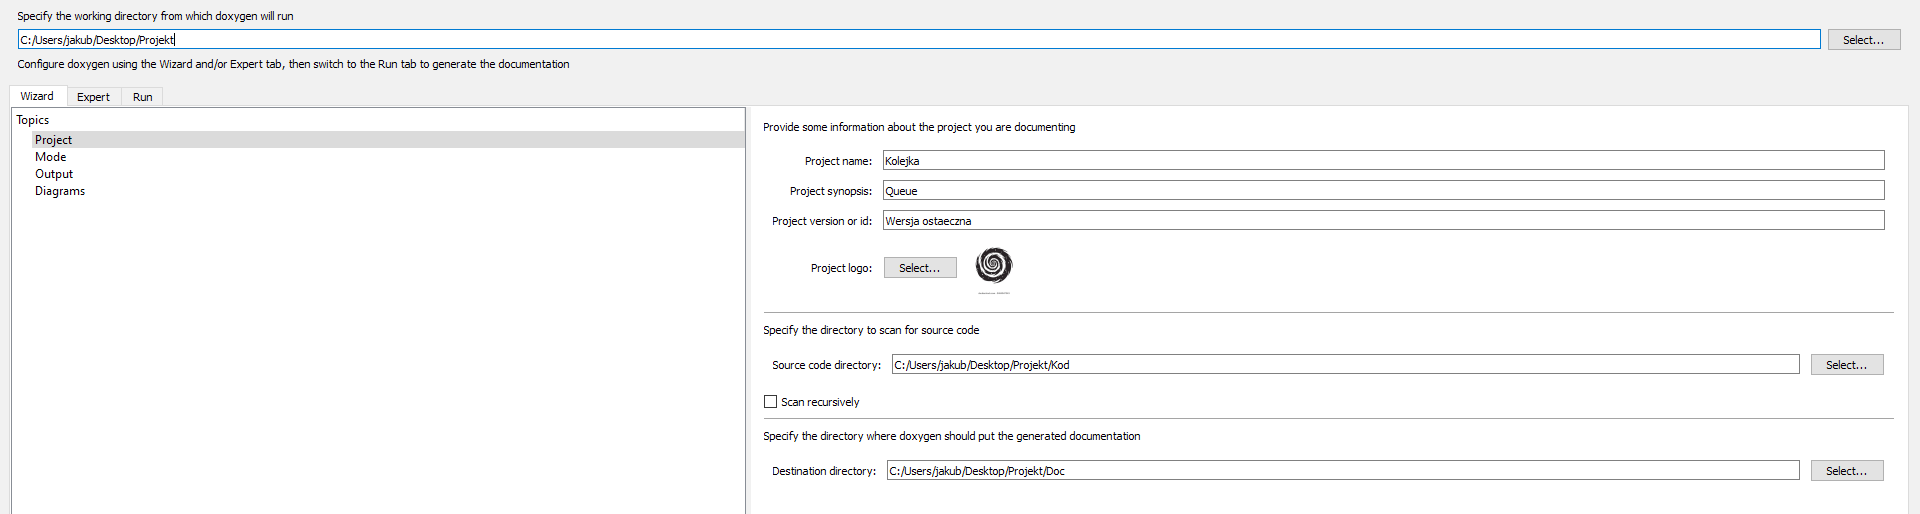
\includegraphics[width=1\textwidth]{images/dox-generacja.png}
    \caption{Okno wizarda doxygen}
\end{figure}

Dzięki wizardowi doxygen, można wygenerować plik konfiguracyjny, który jest niezbędny do wygenerowania dokumentacji. Ułatwia to pracę z doxygenem, a co za tym idzie pozwala na któtszy czas pracy potrzebny do stworzenia dokumentacji.

\begin{figure}[ht]
    \centering
    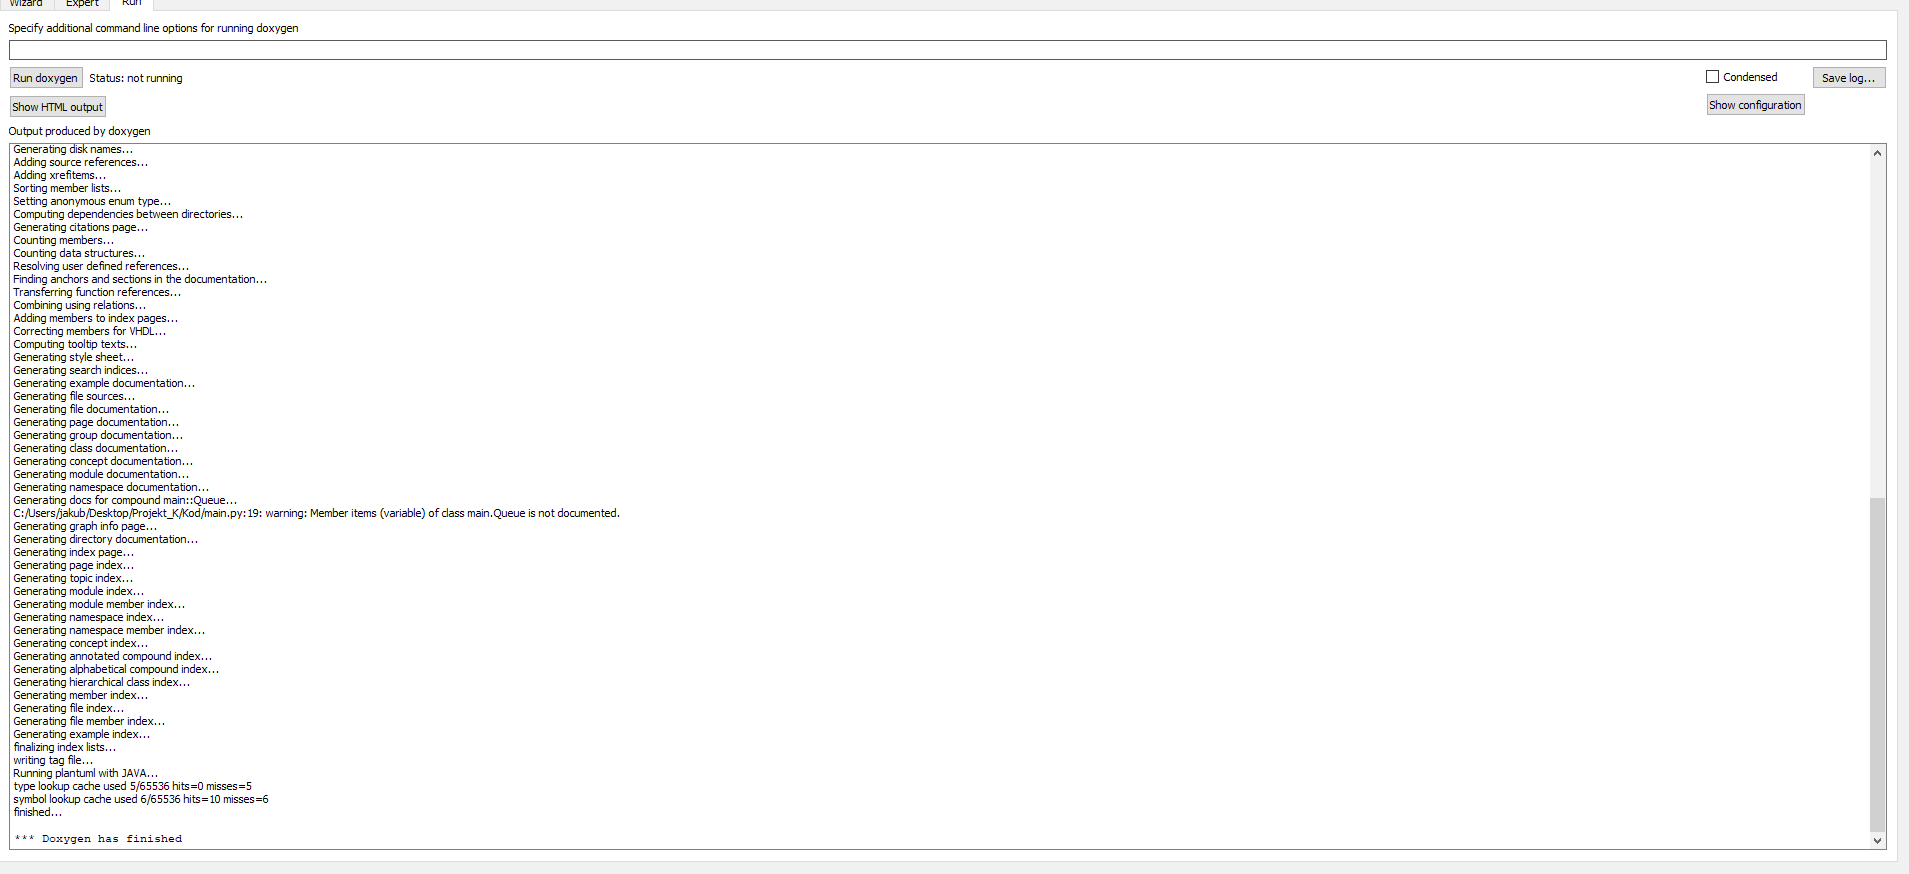
\includegraphics[width=1\textwidth]{images/dox-generacja-2.png}
    \caption{Generacja plików dokumentacji}
\end{figure}

Doxygen szybko generuje pliki dokumentacji, które współpracują
z każdym systemem operacyjnym. W tym przypadku są to pliki HTML, które można otworzyć w dowolnej przeglądarce internetowej.

\newpage
\clearpage

\begin{figure}[ht]
    \centering
    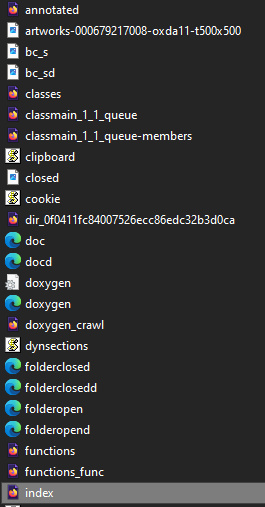
\includegraphics[width=0.5\textwidth]{images/dox-pliki.png}
    \caption{Pliki wygenerowane przez doxygen}
\end{figure}

Aby zobaczyć dokumentację, wystarczy otworzyć plik index.html. W tym przypadku dokumentacja została wygenerowana w języku angielskim, jednak doxygen wspiera wiele języków, w tym również polski; który niestety jest aktualnie ``unmaintained''.

\newpage
\clearpage

\subsection{Dokumentacja}
Jak widać na rysunku \ref{fig:dox-1}, dokumentacja została wygenerowana poprawnie, jest czytelna oraz zawiera wszystko co wprowadziliśmy jako input do wizarda.
\begin{figure}[ht]
    \centering
    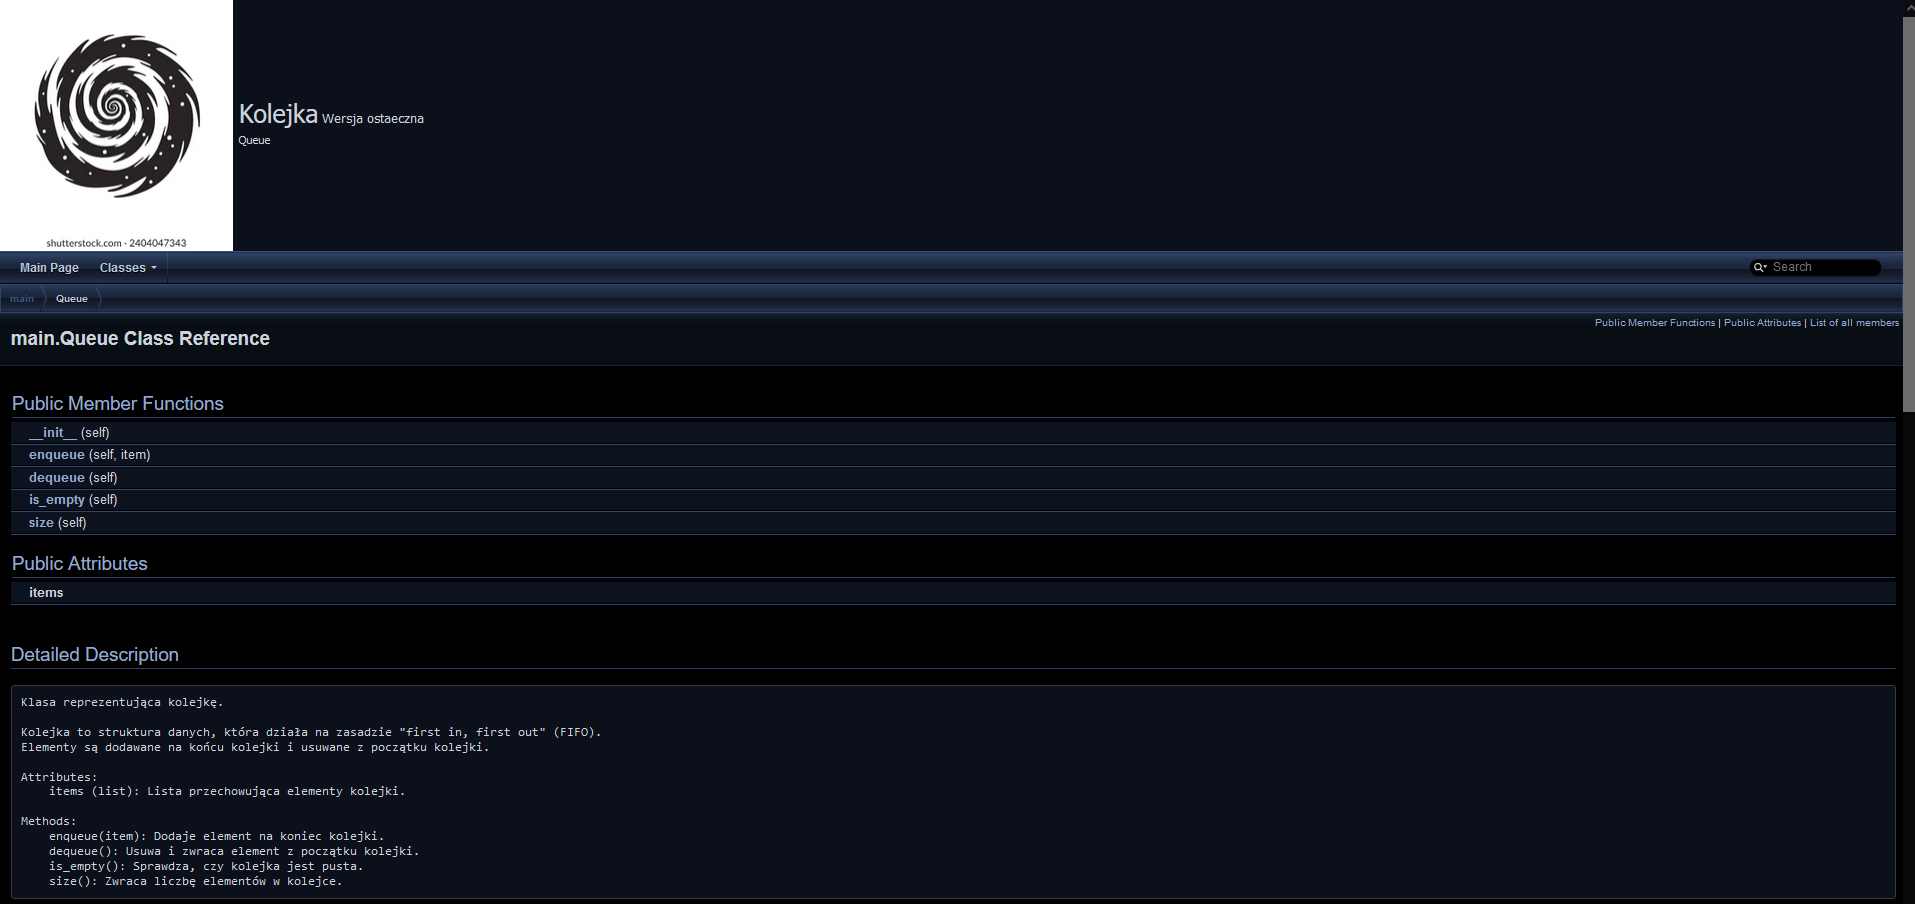
\includegraphics[width=1\textwidth]{images/dox-1.png}
    \caption{Dokumentacja wygenerowana przez doxygen}
    \label{fig:dox-1}
\end{figure}

\begin{figure}[ht]
    \centering
    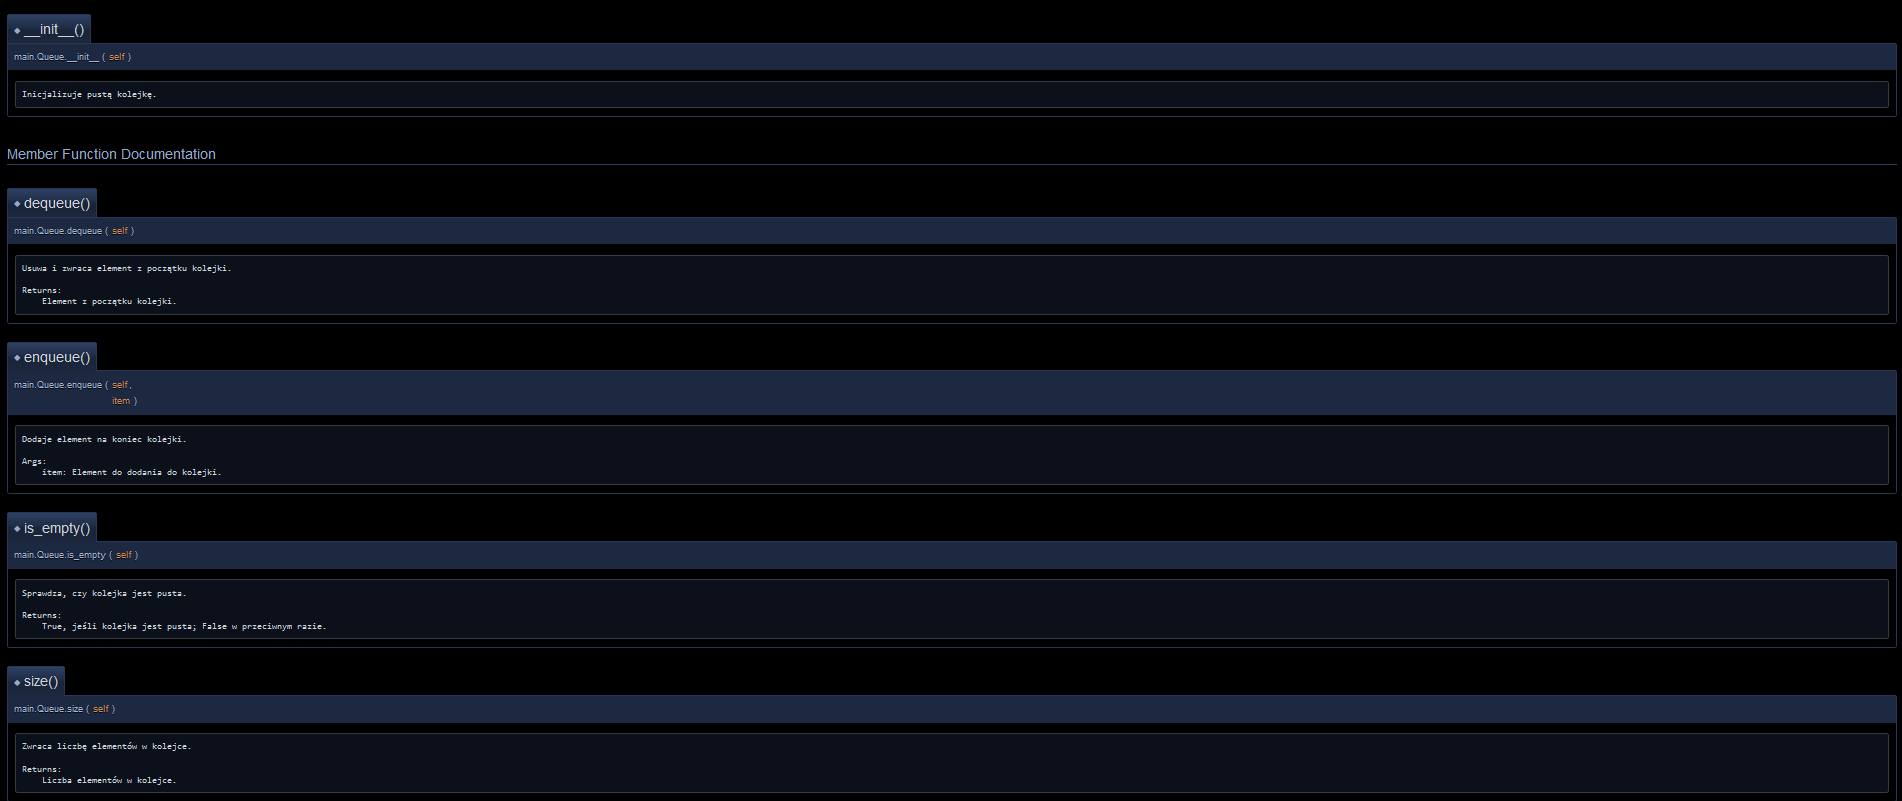
\includegraphics[width=1\textwidth]{images/dox-2.png}
    \caption{Metody klasy Queue w dokumentacji wygenerowanej przez doxygen}
\end{figure}

\newpage
\clearpage

\section{Wnioski}
Po zapoznaniu się z Doxygenem, można stwierdzić, że narzędzie to jest skutecznym rozwiązaniem do automatycznej generacji dokumentacji kodu. Jego integracja z kodem źródłowym oraz możliwość generacji różnych formatów dokumentacji sprawiają, że jest to praktyczne narzędzie dla programistów. Bogate opcje konfiguracyjne oraz wsparcie dla diagramów klas dodają elastyczności i usprawniają proces tworzenia czytelnej dokumentacji.

Nie zmienia to jednak faktu, że doxygen posiada wady. Jedną z nich jest fakt braku wsparcia dla języka polskiego, który jednakże może ulec zmianie. Doxygen również, zdaniem wokalnej części programistów, wymaga ``zaśmiecenia'' kodu źródłowego komentarzami, które są niezbędne do wygenerowania dokumentacji.

Wnioskując, Doxygen jest wartościowym narzędziem dla projektów wymagających zwięzłej i aktualnej dokumentacji kodu, które są w stanie pominąć jego wady.

\printbibliography[title={Bibliografia}, heading=bibintoc]
\nocite{*}

\end{document}